\documentclass[11pt]{article}

\usepackage{apacite}
\usepackage{subcaption}
\usepackage{graphicx}
\usepackage{amsmath}
\usepackage{relsize}
\usepackage{natbib}
\usepackage{float}
\usepackage[margin=1in]{geometry}

\floatstyle{boxed}
\restylefloat{figure}

\title{APPHYS293 Research Project: Theory of Analogy Emergence in Neural Networks}
\author{Andrew Lampinen (lampinen@stanford.edu)}
\date{}
\begin{document}

\maketitle

\section{Introduction}
It is a fascinating feature of neural networks that they are able to respond in sophisticated and subtle ways to multiple related tasks. In particular, one line of work shows that neural networks are capable of extracting analogous structure from knowledge domains that are completely non-overlapping in their inputs and outputs \citep{Hinton1986,Rogers2008a,Lampinen2017}. This extraction of shared structure sets neural networks apart from simple forms of statistical pattern recognition \citep{Rogers2008a}, such as linear data analysis techniques like PCA, which are unable to extract this kind of structure (see below). \par 
Is this feature of neural network learning important? There are a number of reasons to think that it might be. First, recent work has shown that neural networks can show increased performance on a single task from training on multiple related tasks. For example, training a natural language translation system on image captioning and autoencoding improves translation performance \citep{Luong2016}. Learning on numerous language translation pairs can even give generalization without further training to unseen language pairs \citep{Johnson2016a}. (For more multi-task learning examples see e.g.\ \citep{Dong2015,Rusu2015}.) Clearly some aspect of the shared structure between the tasks is contributing to success in these cases. \par 
Furthermore, while multi-task learning is a specific case, it is true more generally that a neural network working on ostensibly a ``single'' task is usually solving multiple tasks with a great deal of structure in common. For example, a network trained to solve the ImageNet classification problem will be trying to identify both monkeys and humans, and there may be many overlapping features it uses to do so. The shared structure between these tasks probably has some impact on learning (for example, the fact that edges are useful for identifying a wide variety of objects may drive the common emergence of Gabor-like filters at the lowest levels of networks trained on ImageNet). \par
Finally, from a cognitive perspective, the human ability to learn from analogous structure between tasks is often considered an essential component of ``what makes us smart'' \citep{Gentner2003}. Although this idea has been attacked at times \cite[e.g.]{Detterman1993}, recent results showing strong implicit analogical transfer effects \cite[e.g.]{Day2011} suggest that these issues may be important to understanding human cognition. \par
\section{Background: a simple task with shared structure}
In previous work \citep{Lampinen2017}, we have shown a surprisingly rich set of phenomena from a very small task, consisting of two perfectly analogous simple tasks. For our task, the inputs can be thought of as the set of letters \(\{R,L,\rho,\lambda\}\), and the outputs as \(\{P,D,S,\pi,\delta,\sigma\}\). The task can be seen as mapping an input letter onto the letters that it can follow (e.g. ``R'' can follow ``D'' as in ``draw,'' but cannot follow ``S''), where there is an analogy between the Latin and Greek letters. See below for the input-output (I/O) mapping:
\[
\begin{array}{c|cccc} 
& R & L & \rho & \lambda \\
\hline
P & 1 & 1 & 0 & 0 \\ 
D & 1 & 0 & 0 & 0 \\
S & 0 & 1 & 0 & 0 \\
\pi    & 0 & 0 & 1 & 1 \\ 
\delta & 0 & 0 & 1 & 0 \\
\sigma & 0 & 0 & 0 & 1 \\
\end{array} 
\]
We \citep{Lampinen2017} solved this task using a variety of linear neural networks, as well as using neural networks with a single nonlinearity (ReLU) at the output layer. We showed that the nonlinear networks are able to access a lower rank solution by exploiting the analogy between the two domains, and qualitatively described why this occurs. \par
Here, I attempt to formalize this qualitative description by using the theory of \citet{Saxe2013}. Although our network is nonlinear, due to the features of the rectifier nonlinearity, at any given point in training, the network and its gradient updates are linear (the units that are below threshold do not contribute to either the outputs or the gradients). Essentially, an input produces a linear pseudo-network as a sub-network of the full network. The catch is that these sub-networks are different for different inputs, but overlap and thus interact. However, in this simple task, it should be possible to characterize linear subnetworks and aggregate changes across them appropriately to completely describe the learning process. \par
\section{Theory}
There have been recent developments in the theory of linear neural networks showing that the process of learning is entirely driven by the Singular Value Decomposition (SVD) of the input-output correlation matrix \citep{Saxe2013}. The SVD can be seen as breaking the structure of the task into individual ``modes'' -- linear structures in the dataset, somewhat like components in PCA. Specifically, a mode consists of an input pattern (which can be interpreted in this case as the input letters the mode responds to), a singular value (which roughly corresponds to the amount of variance explained by this mode), and an output mode (the output letters produced by the given pattern on the inputs). See Fig. \ref{regular_SVD_figure} for the SVD of the I/O mapping for the letter task above. \par
This decomposition tells us more about the task structure the linear network is using to solve the task. There are three modes in the SVD. The first two (left two output modes/top two input modes) represent the base rates of outputs for the within-domain inputs. The first mode maps treats activation of the \(\rho\) or \(\lambda\) inputs identically, and maps it to the \(\pi\) output being on, and the \(\delta\) and \(\sigma\) outputs being half on. The second component performs the same mapping for the Latin letters. The next two components represent the distinctions between the letters \(\rho\) and \(\lambda\) and the letters R and L, respectively. \citet{Saxe2013} showed these results have implications for the learning of non-linear networks as well, so linear neural networks can be a more tractable place to analyzee learning dynamics. In addition, using the I/O SVD allows the discovery of representational components which are distributed across units, so it is more general than simply examining what aspects of the task individual hidden units represent, or examining the weight matrices directly. Thus one might hope to answer our questions in a linear framework. \par
However, linear networks cannot represent analogous structure from non-overlapping inputs and outputs at convergence. With non-overlapping inputs and outputs, the I/O correlation matrix is block diagonal, and the SVD modes will thus occur within blocks (this is why in Fig. \ref{regular_SVD_figure} the modes showing separation between the letters in each domain have no input or output weights to the other domain).\footnote{Where there are duplicated singular values, the SVD is not unique, so more precisely we mean there exists a basis in which the SVD is block diagonal.} Thus, since the final representational components that a linear network learns are precisely the components of the SVD \citep{Baldi1989,Saxe2013}, there will be no sharing of structure across domains.\par 
Furthermore, the optimal rank $k$ approximation to a matrix is to take the top $k$ components from the SVD \citep{Mirsky1960}. If a linear network's hidden layers are restricted to rank lower than that of the I/O correlation matrix, detail within the domains will be lost. Thus a linear neural network cannot solve the task perfectly if any of its hidden layers has a number of units smaller than the rank of the I/O correlation matrix. By contrast, a non-linear network may be able to exploit the analogy between the domains to find more parsimonious solutions.  
\section{Applying the theory to our simple task}
\subsection{Previous results}
\begin{figure}
\centering
\begin{subfigure}{0.22\textwidth}
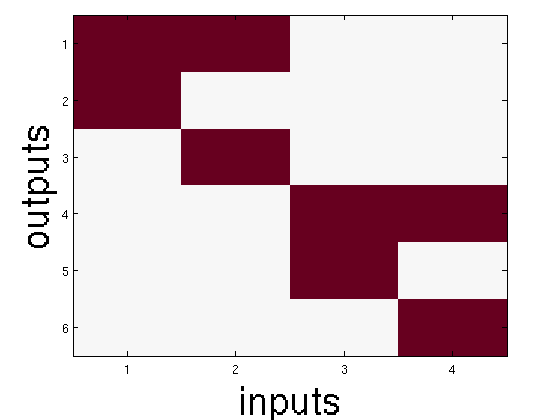
\includegraphics[width=\textwidth]{figures/nonlinear_IO.png}
\caption{I/O mapping}
\label{nonlinear_IO_sub}
\end{subfigure}
\hspace{-0.25em}\LARGE{$=$}\hspace{-0.25em}
\begin{subfigure}{0.22\textwidth}
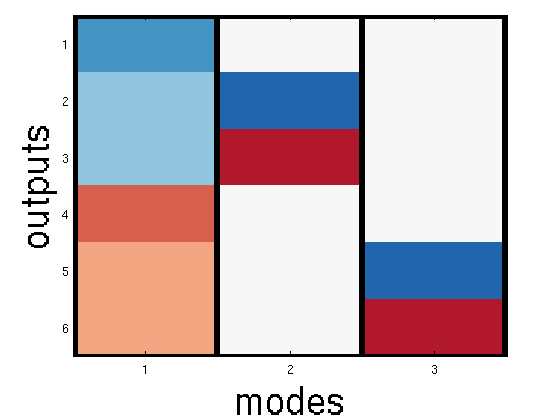
\includegraphics[width=\textwidth]{figures/U_nl.png}
\caption{Output modes $U_{nl}$}
\end{subfigure}
\hspace{-0.25em}\LARGE{$\times$}\hspace{-0.25em}
\begin{subfigure}{0.22\textwidth}
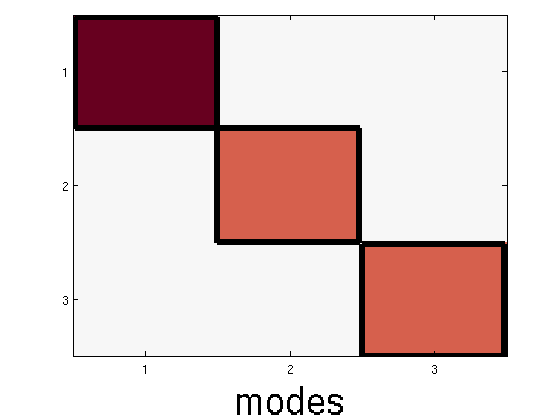
\includegraphics[width=\textwidth]{figures/S_nl.png}
\caption{Singular values $S_{nl}$}
\end{subfigure}
\hspace{-0.25em}\LARGE{$\times$}\hspace{-0.25em}
\begin{subfigure}{0.22\textwidth}
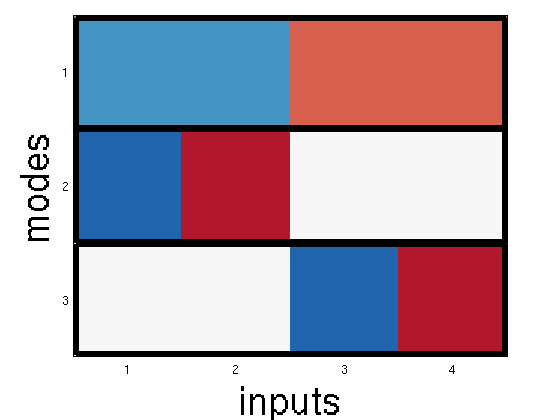
\includegraphics[width=\textwidth]{figures/V_nl.png}
\caption{Input modes $V_{nl}$}
\end{subfigure}
\caption{SVD of I/O correlation matrix (colors are scaled to show qualitative features, red = +, white = 0, blue = -)}
\label{regular_SVD_figure}
\end{figure}
\begin{figure}
\centering
\begin{subfigure}{0.22\textwidth}
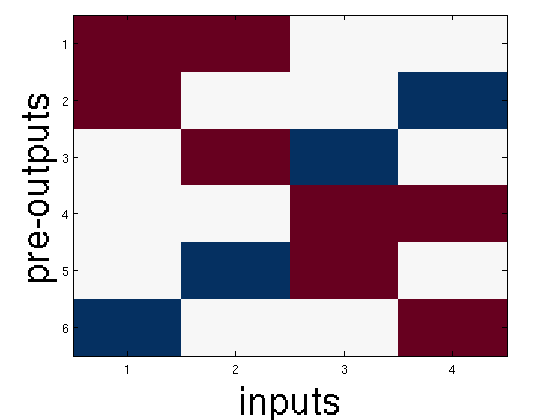
\includegraphics[width=\textwidth]{figures/linearized_IO.png}
\caption{I/O mapping}
\label{linearized_IO_sub}
\end{subfigure}
\hspace{-0.25em}\LARGE{$=$}\hspace{-0.25em}
\begin{subfigure}{0.22\textwidth}
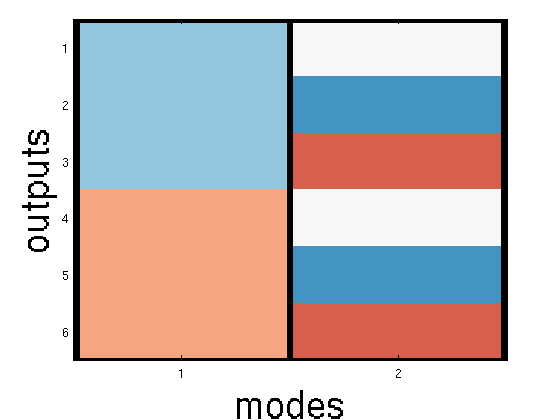
\includegraphics[width=\textwidth]{figures/U_lz.png}
\caption{Output modes $U_{lz}$}
\end{subfigure}
\hspace{-0.25em}\LARGE{$\times$}\hspace{-0.25em}
\begin{subfigure}{0.22\textwidth}
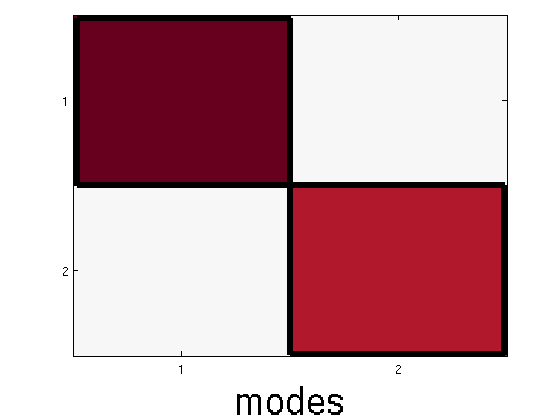
\includegraphics[width=\textwidth]{figures/S_lz.png}
\caption{Singular values $S_{lz}$}
\end{subfigure}
\hspace{-0.25em}\LARGE{$\times$}\hspace{-0.25em}
\begin{subfigure}{0.22\textwidth}
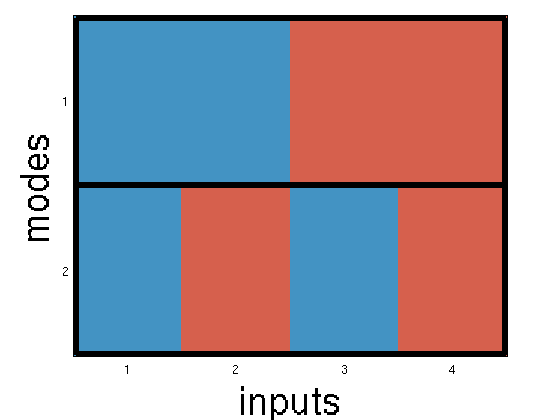
\includegraphics[width=\textwidth]{figures/V_lz.png}
\caption{Input modes $V_{lz}$}
\end{subfigure}
\caption{SVD of linearized I/O correlation matrix (colors are scaled to show qualitative features, red = +, white = 0, blue = -). Note how Fig. \ref{linearized_IO_sub} becomes Fig. \ref{nonlinear_IO_sub} if the negative values are hidden by a rectifier.} 
\label{linearized_SVD_figure}
\end{figure}
Because a linear network cannot extract shared structure, we previously suggested using a network with a non-linearity only at the output, which allows analyses of the SVD to be applied to the linear portion of the network \citep{Lampinen2017}. Although the theory of the dynamics of linear network learning does not apply, we showed that it is still possible to gain some insight into the solutions the network is reaching in this way. \par
Specifically, we found that the network was usually solving the problem by developing a partial offset structure in which it produced a similar pattern of outputs in both domains, but simply offset the ``wrong'' domain sufficiently negative that the pattern of activity would be hidden by the nonlinearity (see Fig. \ref{linearized_IO_sub} for the qualitative pattern). In the ``off'' domain, the output which always responded would be set to \(-1\), and the differential outputs would be set to 0 or \(-1\), if their analogous outputs were 1 and 0, respectively. In this way the network exploits the analogy between the domains while still producing the correct output pattern after the nonlinearity. (Note that due to the symmetry between the two elements of each domain, the network could learn either of the two analogies between them. In practice we observed both, but our analyses here will focus on a single one for clarity.) \par
How does this altered input-output mapping alter the computations the network must perform? When we consider the SVD of this mapping (Fig. \ref{linearized_SVD_figure}), we see that the solution has changed in several ways from the linear I/O mapping (Fig. \ref{regular_SVD_figure}). The modes now treat domains either symmetrically or anti-symmetrically, rather than occurring within domains independently. Rather than two modes for domain selection and two for the structure within each domain, we now observe a single mode for domain selection and a single mode for within-domain structure. The rank of the solution has been reduced from 4 to 2, and thus a neural network with a nonlinearity will only require two hidden units to solve the task, whereas a linear network will require four. This parsimony is achievable because of the analogy between the domains. \par 
We furthermore showed an interesting empirical pattern wherein \textbf{both} a linear and nonlinear network learning the task begin to show some representation of the shared structure early in learning (as measured by projections from the inputs of one domain onto the appropriate outputs of the other domain), but the linear network extinguishes this activity as learning progresses, as it must to reach its final solution of the components of the SVD \citep{Baldi1989,Saxe2013}. By contrast, the nonlinear network stabilizes this output pattern and maintains the analogy between the domains. We were able to describe the dynamics that give rise to this pattern in terms of both a reduction in the mean-squared error and in terms of gradient descent under certain mild assumptions about the weight initializations (that they were not all orthogonal to the analogy pattern). \par
\subsection{New developments}
In this paper, we attempt to build on these results by investigating them more formally. We begin with the following observation: in networks that only use a rectifier nonlinearity, on any given forward pass the network can be seen as behaving like a linear sub-network of itself. Each nonlinearity either shuts a unit off, or passes its input on unaltered. Similarly, the gradients will either be passed linearly, or stopped (the gradient of an ``off'' rectifier is 0). Thus the portion of the network that is active always behaves linearly. Because of this, it might be possible to apply linear network theory in a piecewise fashion to understand the learning dynamics on this task. This is difficult, however, because the sub-network that is active will generally be different on different examples. However, we think that some traction may be gained by analyzing what happens within different examples and how these changes will aggregate. We will perform our analysis within several regimes: \par 
\subsubsection{The linear regime}
Consider the beginning of learning. We initialized our networks with small random positive weights. Since all inputs are \(+1\) or \(0\), the network always begins learning in a completely linear regime. This means that we may apply the results of \citet{Saxe2013} and conclude that (to good approximation), that the first modes to be learned will be those with the largest singular values. \par 
The two modes of the SVD of the I/O mapping that correspond to the base rates by domain have the maximum singular value (see Fig. \ref{regular_SVD_figure}). These modes are (numbers rounded):
\[
\left[ \begin{array}{cc} 
0   & -.8 \\
0   & -.4 \\
0   & -.4 \\
-.8 & 0 \\
-.4 & 0 \\
-.4 & 0 
\end{array} \right]
\times
\left[ \begin{array}{cc} 
1.7 & 0 \\
0 & 1.7 
\end{array} \right]
\times
\left[ \begin{array}{cccc} 
-.7 & -.7 & 0 & 0 \\ 
0 & 0 & -.7 & -.7 
\end{array} \right]
\]
However, because these modes have the same singular value, the SVD is non-unique in the sense that any orthogonal linear combination of these two modes creates an equally valid SVD. Consider the basis: 
\[
\left[ \begin{array}{cc} 
.6   & -.6 \\
.3  & -.3 \\
.3  & -.3 \\
.6 & .6 \\
.3 & .3 \\
.3 & .3 
\end{array} \right]
\times
\left[ \begin{array}{cc} 
1.7 & 0 \\
0 & 1.7 
\end{array} \right]
\times
\left[ \begin{array}{cccc} 
.5 & .5 & .5 & .5 \\
.5 & .5 & -.5 & -.5 
\end{array} \right]
\]
In this basis, the first mode corresponds to the overall base rate activation of the output units, and the second to the base rates by domain. Interestingly, we observed in our previous paper (and others have observed previously) that the base rates are consistently learned very rapidly, prior to the base rates by domain correction, despite the fact that they have the same singular values. This occurs even though they explain the same amount of variance in the final mapping (since they have the same singular value), and despite the fact that learning either of them would result in the same change in the MSE. (Note that in a standard neural network this would occur because of the biases, but we did not use biases to simplify the analysis and avoid confounds like this.) \par 
This initially puzzled us, since it occurs in the linear regime but was out of keeping with the basic predictions of Saxe and colleagues. However, upon reflection it is clear that our small positive initialization is biased to have a greater projection onto the first component than the second. Saxe and colleagues derived the time to learn a mode to be:
\[t = \frac{\tau}{2s} \ln \frac{u_f(s-u_0)}{u_0(s-u_f)}\]
where \(u_0\) is the initial projection. Thus, as \(u_0\) increases, learning time goes down, so the bias in order of learning we observed is presumably due to this biased initialization. To confirm this, we trained a linear network initialized with weights normally distributed with mean zero, and as expected the components were learned at approximately the same time in this case. \par
The small positive initialization we chose is convenient for us, however, since it means that both the first two components are learned within the linear regime. Once the second component is learned, however, the network begins to hit the nonlinearity in the ``off'' domain, leading to the second learning regime, which we discuss in the next section.\par
\subsubsection{Alternating domains regime}
Once the first two components of the linear SVD have been learned, the network will begin to hit the non-linearity in the ``off'' domain, and thus will leave the linear learning regime. Instead, the network now has two modes: a Latin mode whenever a Latin input comes in, where the Latin outputs are the within-domain base rates of the Latin units, and the Greek units are off, and an analogous mode for the Greek inputs. These correspond to two sub-networks which essentially just omit the output units for the ``off'' domain. \par
Within these sub-networks, what needs to be learned? Consider the Latin sub-network. The only remaining component of the SVD for this sub-network is the mode corresponding to the distinction between the letters R and L. Thus, the learning of this component will proceed, and analogously for the Greek domain letters \(\rho\) and \(\lambda\). \par
However, there is a crucial difference from linear networks at this point. Because these modes are being learned within sub-networks, they will not exhibit the competition between connectivity modes that occurs in linear networks according to the theory of Saxe and colleagues. This means that the modes will not feel a ``force'' which is trying to orthogonalize them in the hidden unit representational space. \par
Of course, as soon as these modes accumulate any appreciable strength, some of the ``off'' units will start to turn on again, and the sub-networks will grow more complicated. This lead to the next regime: \par
\subsubsection{Domains + a bit of analogy regime}    
In this regime, each input results in its own subnetwork. A letter turns on the outputs from its language with their base rates plus a small amount of the within domain distinction, and a small amount of analogy to the letters in the other domain. To make this more concrete, the I/O mapping (prior to the nonlinearity) will look something like the following:
\[
\left[ \begin{matrix} 
 1 & 1 & 0 & 0 \\ 
 0.6 & 0.4 & 0.1 & -0.1 \\
 0.4 & 0.6 & -0.1 & 0.1 \\
 0 & 0 & 1 & 1 \\ 
  0.1 & -0.1 & 0.6 & 0.4 \\
  -0.1 & 0.1 & 0.4 & 0.6 \\
\end{matrix}  \right] 
\]
Thus in addition to the within-domain outputs, the analogous output in the ``off'' domain will be slightly activated. This will reintroduce interference between the modes. The network can resolve this in two ways: 
\begin{enumerate}
\item Reducing the output of the analogous output in the ``off'' domain, without adjusting the other ``off'' domain outputs. 
\item Shifting the balance between the first two modes of the linear SVD so that the ``off'' domain as a whole is offset more negative. (This is an acceptable solution only with the nonlinearity, of course.)
\end{enumerate} 
Which of these solutions will the network follow? Both result in a reduction in the MSE, and there is pressure toward both the first from each input individually, the second from aggregating across the different inputs. Thus we might expect the network to follow both solution paths. This predicts that in the final solutions, the pre-outputs for the non-analogous off-domain letter will be more negative than those for the always-on off-domain letter, because the non-analogous letter is being made more negative by both these mechanisms, while the always-on letter is only being affected by the latter. Indeed, we observe these results (post-hoc) in 95 of our 100 runs (in the five runs where we didn't observe it, in four cases it was still true for three of the four inputs, and in the 5th it was true for two of the four).\par
Once the network has started to incorporate these changes, the ``off'' domain will be shut off again, and the network will shift back to the alternating domains regime. When the analogous ``off''-domain letter is outputting zero, there should be no impetus to reduce it or the other outputs of the domain further. Thus we would expect the outputs for the analogous letter to always be close to zero, and indeed we observed this (post-hoc) on 95 of our 100 runs (the 5 runs where we didn't observe it did not overlap with the 5 from above, and in all these cases the prediction still held true for three of the four inputs). \par 
Of course, when the network switches back to the alternating domains regime, it will again develop representations that push it into this regime, so the network will oscillate between representing the analogy and suppressing it until the task is learned.
\subsubsection{Summary and further results}
In summary, we believe this is the general process by which our network develops solutions that reflect the analogy:
\begin{enumerate}
\item The network begins learning linearly, and learns the base rates of the units and then the base rates by domain. 
\item At this point, the network switches to a non-linear regime in which each domain is shut off when it is supposed to be off. At this point, unlike the linear case, there is no competition between the modes, so they will end up overlapping to some extent, which will result in the network learning some of the analogy. 
\item Once the analogy has been slightly learned, the network will switch to a regime where the analogous unit from the ``off'' domain is slightly active, which will reintroduce some competition between the modes. The network will resolve this by suppressing the analogous output and the whole domain, and thus switch back to the previous regime.
\item The network will oscillate between these regimes until convergence.
\end{enumerate}
Although this explanation is still not completely formal, it is developed enough to allow us to understand the behavior of the network better, and to make predictions about its performance that we were unable to previously.\par
First, this explanation makes clear predictions about how rank of the network impacts solutions. It suggests that the emergence of an analogy in the case when the hidden layer has four hidden units is in some ways a coincidence -- it emerges because there is not competition between the modes for the different domains to orthogonalize them, rather than because of some force that drives its extraction. This makes the prediction that in a network with a very large hidden layer, there should be very little representation of the analogy, because the modes won't overlap since random vectors are close to orthogonal in high dimensional spaces. We evaluated this prediction by training networks with a 1000 unit hidden layer, and indeed we see no evidence of significant representation of the analogy within any of these runs. \par
This explanation also clarifies why the analogy emerges consistently in the case where the network is only given two hidden units, and thus must discover it to solve the task. In the case of a 2-dimensional representation space, once the mode for the domain switching is learned, the other modes will be ``squeezed'' into the single orthogonal mode in the space (since they compete with the domain switching mode, but not with each other, as above). Thus the extraction of the analogy is most complete when the network is forced to find low-rank solutions to the task.\par
\section{Conclusions \& Future Directions}
We set out to explore the results of \citet{Lampinen2017} in greater detail, and have outlined a more complete description of why they occurred. We suggest that these results occurred in effect because the nonlinearity allows domains to be shut off, and thus reduces competition between the modes for the within domain structure, allowing them to remain non-orthogonal. This suggests that analogy is most likely to emerge from trying to find low-rank solutions to a problem.\par
However, this may only be true if the network is assumed to have a single hidden layer. This is a fairly artificial assumption, since the human brain is deep and richly recurrent. With deeper networks where weights are shared between the tasks, there may be more force that causes extraction of analogies, since the networks can share connectivity modes in the hidden layer to hidden layer connections. Essentially, a mode that represents analogous structure should explain more variance than one that does not, so one might hope it would be extracted sooner. This would be an exciting direction for future research.  \par
Our results also provide potential directions to search for the methods that humans use to find analogies. In general, finding analogical mappings can reduce to a difficult graph or subgraph isomorphism problem, resulting in worst-case runtimes of \(O(n!)\) for even relatively sophisticated systems, e.g. \citet{Falkenhainer1989}. Humans are often quite fast at recognizing these analogies, however. Is it possible that we do so by attempting to find low-rank solutions to the problem of representing these domains? If humans amortize this inference over the longer timescales of interacting with the analogy domains, this might explain our ability to make fast symbolic mappings between them. This idea makes specific predictions about deficits in making analogical mappings with domains that subjects have little experience with (especially if this experience was e.g. by listening to lectures rather than by interacting with the concepts), which could be tested in future work. \par
It would also be interesting to attempt to address the benefits of multi-task learning for neural networks from a similar perspective. Under what circumstances are multiple tasks beneficial? Does this depend in a similar fashion on the size of the hidden layer, or are the dynamics different in deeper networks where computations are shared? \par 
In exploring these questions (and many others), the analysis technique of treating rectifier networks as networks that are learning linearly on any given example could prove beneficial. The technique could be applied with few changes to networks of arbitrary depth, although the pattern of switching would grow more complex. It might be possible to automate the analysis by creating a system which observes the network's performance on different examples and then computes the next point when a unit will switch from on to off or vice versa, and then to compute the linear solutions from this point and so on. This could potentially allow for a more complete understanding of how neural networks solve tasks.\par 
\bibliographystyle{apalike}
\bibliography{shared_reps}


\end{document}
